\chapter{Ověřovací měření}


\section{Metodika měření}

Pro ověřovací měření byla použita sada ověřovacích součástek uvedených v tabulce~\ref{tab:overovaci-soucastky}. Každá součástka byla změřena navrženým měřičem a referenčním LCR metrem.

Každá součástka (s vyjímkou rezistoru) byla změřena při frekvencích 1, 10 a 100 kHz. Rezistor a hodnoty sériového odporu součástek byly měřeny při frekvenci 1kHz.
Jako referenční přístroj byl použit ruční LCR metr BK Precision 880, který umožňuje měření parametrů R, L, C. \cite{BKPrecision_880_Datasheet}.

\begin{figure}[H]
    \centering
    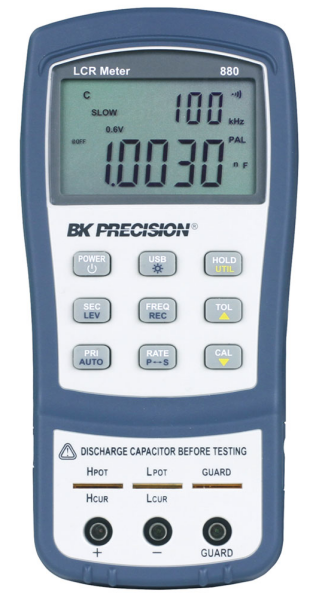
\includegraphics[height=0.30\textheight]{obrazky/BK_precision_880.png}
    \caption{Referenční LCR metr BK Precision 880. Převzato z \cite{BKPrecision_880_Datasheet}.}
    \label{fig:bk_precision_880}
\end{figure}

Nastavování amplitudy měřicího signálu, bočníku a zesilovačů bylo pro každé měření provedeno tak, 
aby měřené signály zabíraly co největší část rozsahu \acs{A/D} převodníků.

Všechny měření byly provedeny s počtem vzorků 1000.

\begin{table}[H]
    \centering
    \small
    \caption{Ověřovací součástky použité při měření.}
    \label{tab:overovaci-soucastky}
    \begin{tabular}{@{}>{\centering\arraybackslash}m{1.85cm} l c l@{}}
        \toprule
        & Součástka & Zkratka & Nominální hodnota \\
        \midrule
        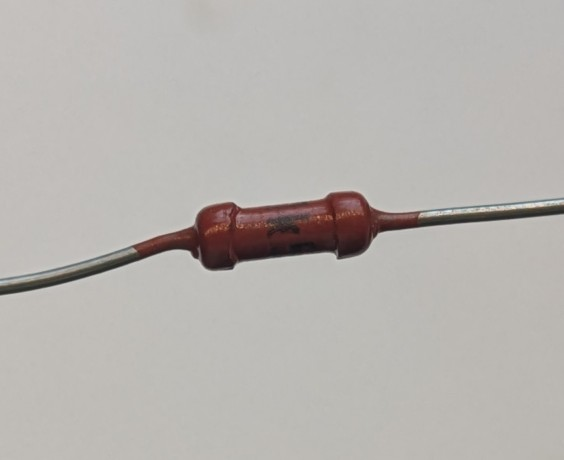
\includegraphics[width=1.5cm,height=1.5cm,keepaspectratio]{obrazky/komponenty/rezistor.jpg} & Rezistor & $R$ & $1{,}5\,\mathrm{k}\Omega$ \\
        \addlinespace[0.25em]
        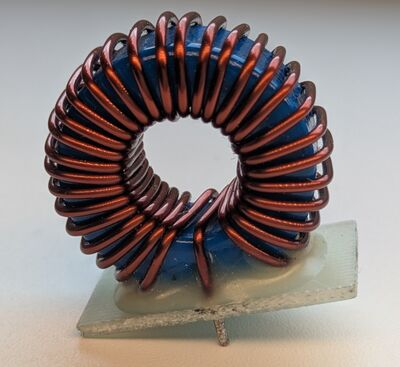
\includegraphics[width=1.5cm,height=1.5cm,keepaspectratio]{obrazky/komponenty/civka_velka.jpg} & Cívka toroidní & $L_{\mathrm{Toroid}}$ & \textit{neznámá} \\
        \addlinespace[0.25em]
        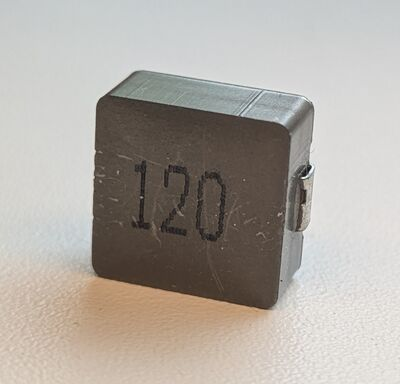
\includegraphics[width=1.5cm,height=1.5cm,keepaspectratio]{obrazky/komponenty/civka_smd.jpg} & Cívka SMD & $L_{\mathrm{SMD}}$ & $12\,\mu\mathrm{H}$ \\
        \addlinespace[0.25em]
        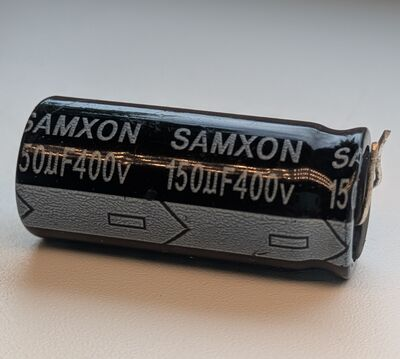
\includegraphics[width=1.5cm,height=1.5cm,keepaspectratio]{obrazky/komponenty/cap_electrolyt.jpg} & Elektrolytický kondenzátor & $C_{\mathrm{Elektrolyt}}$ & $150\,\mu\mathrm{F}$ \\
        \addlinespace[0.25em]
        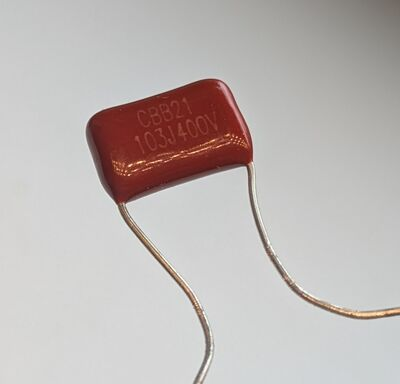
\includegraphics[width=1.5cm,height=1.5cm,keepaspectratio]{obrazky/komponenty/cap_pp_maly.jpg} & Polypropylenový kondenzátor & $C_{\mathrm{10n}}$ & $10\,\mathrm{nF}$ \\
        \addlinespace[0.25em]
        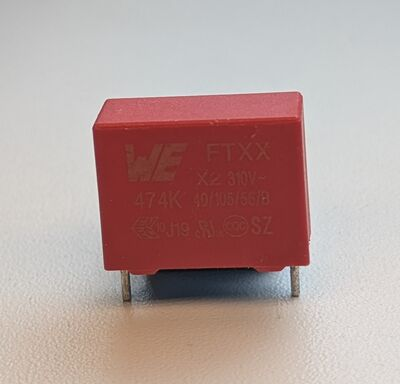
\includegraphics[width=1.5cm,height=1.5cm,keepaspectratio]{obrazky/komponenty/cap_pp_velky.jpg} & Polypropylenový kondenzátor (větší) & $C_{\mathrm{470n}}$ & $470\,\mathrm{nF}$ \\
        \bottomrule
    \end{tabular}
\end{table}


\section{Výsledky měření}

V tabulce~\ref{tab:vysledky-komponenty} jsou uvedeny hodnoty změřené referenčním přístrojem BK Precision 880.
Červeně vyznačené hodnoty nelze brát v potaz, jelikož jsou mimo funkční rozsah přístroje \cite{BKPrecision_880_Datasheet}.

Tabulka~\ref{tab:vysledky-navrh} uvádí hodnoty naměřené navrženým LCR metrem. Hodnota kapacity elektrolytického kondenzátoru při 100 kHz chybí, 
protože při takto vysoké frekvenci přístroj měřil součástku jako induktivní.

K porovnání slouží tabulka~\ref{tab:odchylky} s hodnotami relativní odchylky vypočtenými podle rovnice:

\begin{equation}
    \delta = \frac{X_{\mathrm{navržen}} - X_{\mathrm{referenční}}}{X_{\mathrm{referenční}}} \times 100\,\%
    \label{eq:relativni-odchylka}
\end{equation}

Pro lepší porozumění situaci byly hodnoty měřené při frekvenci 1 kHz vyneseny na číselné osy v obr.~\ref{fig:komponent_viz}

\begin{table}[H]
    \centering
    \small
    \caption{Hodnoty ověřovacích součástek naměřené LCR metrem BK Precision 880. 
    Červeně vyznačené hodnoty jsou mimo funkční rozsah měřicího přístroje.}
    \label{tab:vysledky-komponenty}
    \begin{tabular}{@{}l r c c c@{}}
        \toprule
        Součástka           & $R $       & \multicolumn{1}{c}{1\,kHz}   & \multicolumn{1}{c}{10\,kHz}  & \multicolumn{1}{c}{100\,kHz} \\
        \midrule
        $R$                 & $1{,}454\,\mathrm{k}\Omega$ & ---                         & ---                          & ---                          \\
        \addlinespace[0.35em]
        $L_{\mathrm{Toroid}}$   & $20{,}8\,\mathrm{m}\Omega$  & $107\,\mu\mathrm{H}$        & $107\,\mu\mathrm{H}$         & $106\,\mu\mathrm{H}$         \\
        \addlinespace[0.35em]
        $L_{\mathrm{SMD}}$      & $26{,}1\,\mathrm{m}\Omega$  & $12{,}8\,\mu\mathrm{H}$     & $12{,}8\,\mu\mathrm{H}$      & $12{,}3\,\mu\mathrm{H}$      \\
        \addlinespace[0.35em]
        $C_{\mathrm{Elektrolyt}}$ & $571\,\mathrm{m}\Omega$   & $106\,\mu\mathrm{F}$        & \cellcolor{red!20}$7{,}98\,\mu\mathrm{F}$      & \cellcolor{red!20}$485\,\mathrm{nF}$           \\
        \addlinespace[0.35em]
        $C_{\mathrm{10n}}$      & $2{,}942\,\Omega$          & $9{,}71\,\mathrm{nF}$       & $9{,}71\,\mathrm{nF}$        & $9{,}71\,\mathrm{nF}$        \\
        \addlinespace[0.35em]
        $C_{\mathrm{470n}}$     & $87{,}9\,\mathrm{m}\Omega$  & $455\,\mathrm{nF}$          & $455\,\mathrm{nF}$           & $452\,\mathrm{nF}$           \\
        \bottomrule
    \end{tabular}
\end{table}

\begin{table}[H]
    \centering
    \small
    \caption{Hodnoty ověřovacích součástek naměřené navrženým LCR metrem.}
    \label{tab:vysledky-navrh}
    \begin{tabular}{@{} l
        S[table-format=3.3]@{\,}l
        S[table-format=3.2]@{\,}l
        S[table-format=3.2]@{\,}l
        S[table-format=3.2]@{\,}l @{}}
        \toprule
        Součástka & \multicolumn{2}{c}{$R$}
                   & \multicolumn{2}{c}{1\,kHz}
                   & \multicolumn{2}{c}{10\,kHz}
                   & \multicolumn{2}{c}{100\,kHz} \\
        \midrule
        $R$          & 1.478   & $\mathrm{k}\Omega$ & \multicolumn{2}{c}{---}
                     & \multicolumn{2}{c}{---} & \multicolumn{2}{c}{---} \\
        \addlinespace[0.35em]
        $L_{\mathrm{Toroid}}$
                     & 30.39   & $\mathrm{m}\Omega$ & 109.42 & $\mu\mathrm{H}$
                     & 110.92  & $\mu\mathrm{H}$   & 108.16 & $\mu\mathrm{H}$ \\
        \addlinespace[0.35em]
        $L_{\mathrm{SMD}}$
                     & 31.57   & $\mathrm{m}\Omega$ & 13.22  & $\mu\mathrm{H}$
                     & 12.96   & $\mu\mathrm{H}$   & 12.28  & $\mu\mathrm{H}$ \\
        \addlinespace[0.35em]
        $C_{\mathrm{Elektrolyt}}$
                     & 733.40  & $\mathrm{m}\Omega$ & 126.56 & $\mu\mathrm{F}$
                     & 120.21  & $\mu\mathrm{F}$   & \multicolumn{2}{c}{---} \\
        \addlinespace[0.35em]
        $C_{\mathrm{10n}}$
                     & 43.50   & $\Omega$           & 9.78   & $\mathrm{nF}$
                     & 9.83    & $\mathrm{nF}$     & 9.16   & $\mathrm{nF}$ \\
        \addlinespace[0.35em]
        $C_{\mathrm{470n}}$
                     & 1.31    & $\Omega$           & 452.94 & $\mathrm{nF}$
                     & 449.45  & $\mathrm{nF}$     & 533.39 & $\mathrm{nF}$ \\
        \bottomrule
    \end{tabular}
\end{table}

\begin{table}[H]
    \centering
    \small
    \caption{Relativní odchylky hodnot naměřených navrženým LCR metrem od referenčního měření přístrojem BK Precision 880.}
    \label{tab:odchylky}
    \begin{tabular}{@{} l c c c c @{}}
        \toprule
        Součástka & $R$ & 1\,kHz & 10\,kHz & 100\,kHz \\
        \midrule
$R$ & $1{,}7\,\%$ & --- & --- & --- \\
        \addlinespace[0.35em]
        $L_{\mathrm{Toroid}}$ & $46{,}1\,\%$ & $2{,}3\,\%$ & $3{,}7\,\%$ & $2{,}0\,\%$ \\
        \addlinespace[0.35em]
        $L_{\mathrm{SMD}}$ & $21{,}0\,\%$ & $3{,}3\,\%$ & $1{,}3\,\%$ & $0{,}2\,\%$ \\
        \addlinespace[0.35em]
        $C_{\mathrm{Elektrolyt}}$ & $28{,}4\,\%$ & $19{,}4\,\%$ & $1406\,\%$ & --- \\
        \addlinespace[0.35em]
        $C_{\mathrm{10n}}$ & $1379\,\%$ & $0{,}7\,\%$ & $1{,}2\,\%$ & $5{,}7\,\%$ \\
        \addlinespace[0.35em]
        $C_{\mathrm{470n}}$ & $1390\,\%$ & $0{,}5\,\%$ & $1{,}2\,\%$ & $18{,}0\,\%$ \\
        \bottomrule
    \end{tabular}
\end{table}

\begin{figure}[H]
    \centering
    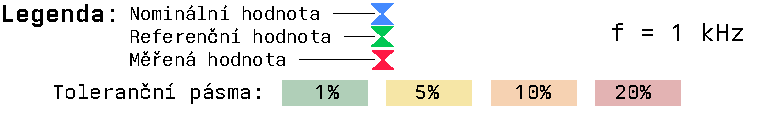
\includegraphics[width=0.93\linewidth]{obrazky/komponent_viz/legend.pdf}
    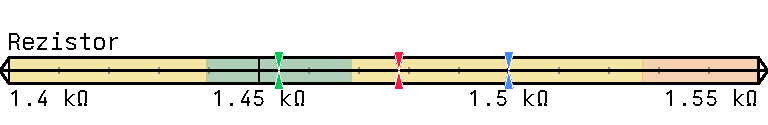
\includegraphics[width=0.93\linewidth]{obrazky/komponent_viz/R_DCR.pdf}

    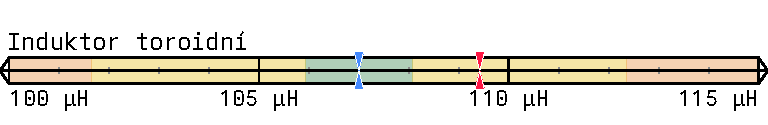
\includegraphics[width=0.93\linewidth]{obrazky/komponent_viz/L_Toroid_1kHz.pdf}

    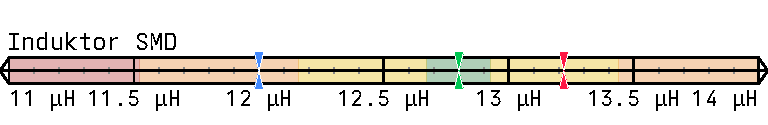
\includegraphics[width=0.93\linewidth]{obrazky/komponent_viz/L_SMD_1kHz.pdf}

    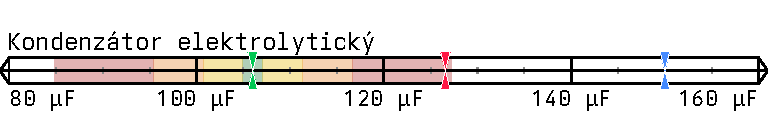
\includegraphics[width=0.93\linewidth]{obrazky/komponent_viz/C_Elektrolyt_1kHz.pdf}

    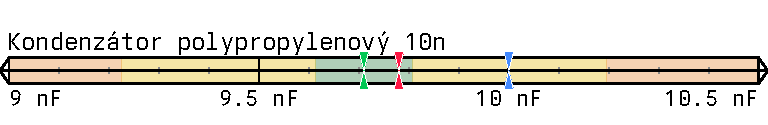
\includegraphics[width=0.93\linewidth]{obrazky/komponent_viz/C_10n_1kHz.pdf}

    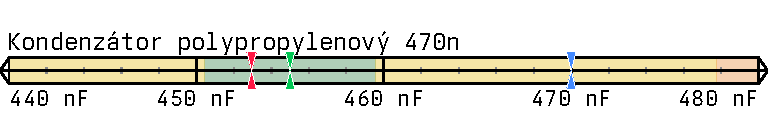
\includegraphics[width=0.93\linewidth]{obrazky/komponent_viz/C_470n_1kHz.pdf}
    \caption{Grafické porovnání hodnot naměřených navrženým LCR metrem a referenčním přístrojem BK Precision 880.}
    \label{fig:komponent_viz}
\end{figure}



\subsection{Stabilita měření}

Ke zjištění stability měření byla použita softwarová funkce mnohonásobného měření.
Tyto měření nebyly porovnány s referenčním LCR metrem, protože ten takovou funkci nemá.

\begin{figure}[H]
    \centering
    
\includegraphics[width=0.48\linewidth]{obrazky/komponent_viz/histogramy/toroid_1khz_L.pdf}
    
\includegraphics[width=0.48\linewidth]{obrazky/komponent_viz/histogramy/toroid_1khz_R.pdf}
    \caption{Histogramy hodnot $L_{\mathrm{Toroid}}$ a jeho sériového odporu při $1\,\mathrm{kHz}$}
    \label{fig:histogram_toroid_1khz}
\end{figure}

\begin{figure}[H]
    \centering
    
\includegraphics[width=0.48\linewidth]{obrazky/komponent_viz/histogramy/toroid_10khz_L.pdf}
    
\includegraphics[width=0.48\linewidth]{obrazky/komponent_viz/histogramy/toroid_10khz_R.pdf}
    \caption{Histogramy hodnot $L_{\mathrm{Toroid}}$ a jeho sériového odporu při $10\,\mathrm{kHz}$}
    \label{fig:histogram_toroid_10khz}
\end{figure}

\begin{figure}[H]
    \centering
    
\includegraphics[width=0.48\linewidth]{obrazky/komponent_viz/histogramy/toroid_100khz_L.pdf}
    
\includegraphics[width=0.48\linewidth]{obrazky/komponent_viz/histogramy/toroid_100khz_R.pdf}
    \caption{Histogramy hodnot $L_{\mathrm{Toroid}}$ a jeho sériového odporu při $100\,\mathrm{kHz}$}
    \label{fig:histogram_toroid_100khz}
\end{figure}

\begin{figure}[H]
    \centering
    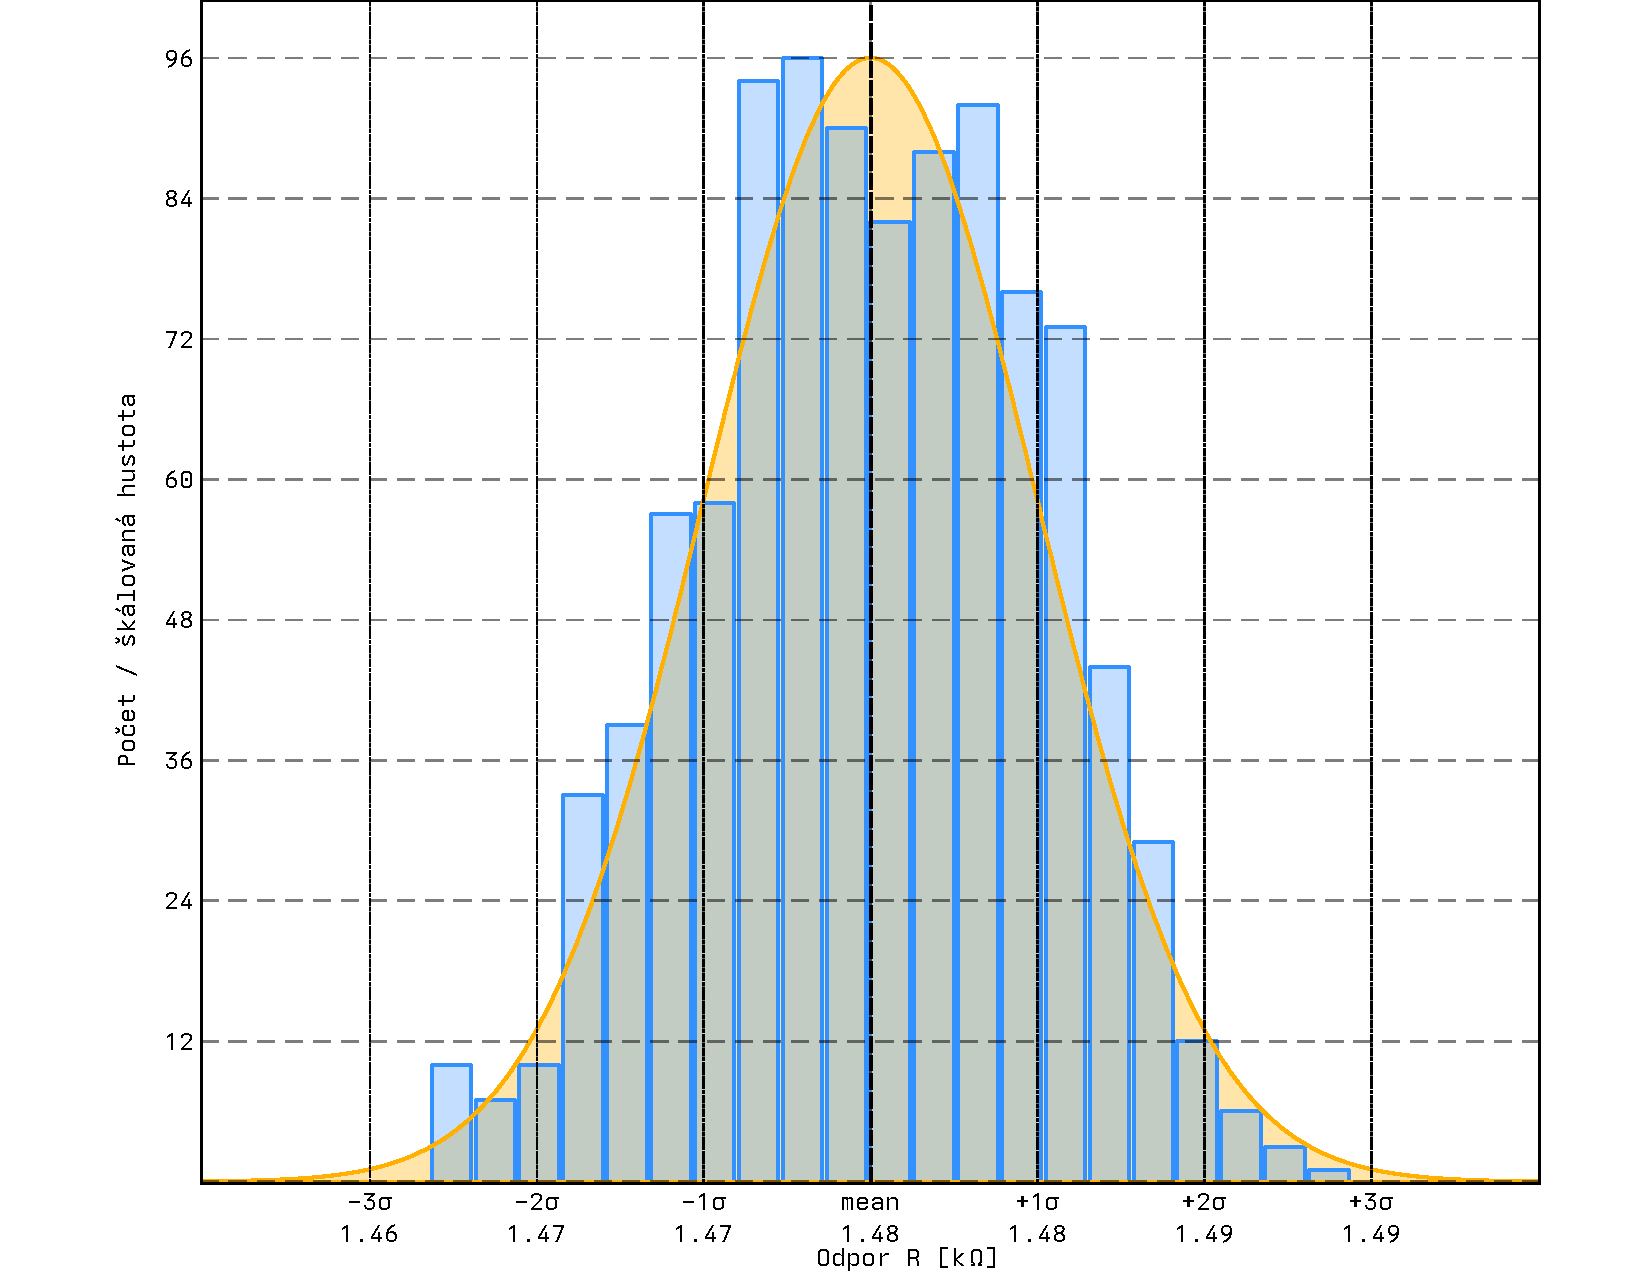
\includegraphics[width=0.48\linewidth]{obrazky/komponent_viz/histogramy/R_10khz.pdf}
    
\includegraphics[width=0.48\linewidth]{obrazky/komponent_viz/histogramy/r_phase_diff_10khz.pdf}
    \caption{Histogramy hodnot odporu a fázového rozdílu rezistoru při $10\,\mathrm{kHz}$}
    \label{fig:histogram_rezistor}
\end{figure}

\begin{table}[H]
    \centering
    \caption{Směrodatné odchylky měření toroidní cívky}
    \label{tab:histogram_smerodatne_odchylky}
    \begin{tabular}{lcc}
        \toprule
        Frekvence & $\sigma(L)$ [$\mu$H] & $\sigma(R)$ \\
        \midrule
        $1\,\mathrm{kHz}$   & $0{,}77$ & $7{,}12\,\mathrm{m}\Omega$ \\
        $10\,\mathrm{kHz}$  & $0{,}34$ & $21{,}3\,\mathrm{m}\Omega$  \\
        $100\,\mathrm{kHz}$ & $1{,}22$ & $0{,}70\,\mathrm{\Omega}$   \\
        \bottomrule
    \end{tabular}
\end{table}

\section{Diskuze výsledků}

Z dosažených výsledků ověřovacích měření vyplývá, že navržený digitální měřič impedance úspěšně plní svou základní funkci a ve většině provozních režimů dosahuje stanovených cílů. 

Při měření polypropylenových kondenzátorů ($C_{10n}$ a $C_{470n}$) vykazuje přístroj excelentní shodu s referenčním LCR metrem BK Precision 880, kdy relativní odchylka kapacity nepřekročila hranici 1~\% v celém pásmu do 10~kHz. Velmi dobrých výsledků v rámci stanoveného tolerančního pásma do 5~\% bylo dosaženo také u charakterizace induktorů ($L_{Toroid}$ a $L_{SMD}$) a kalibračního rezistoru.

\subsection{Statistická stabilita a chování na nízkých kmitočtech}
Při měřicích frekvencích 1~kHz a 10~kHz odpovídá rozdělení naměřených hodnot v histogramech standardnímu normálnímu (Gaussovu) rozdělení, což potvrzuje, že dominantním zdrojem nejistoty je v těchto oblastech náhodný šum. Na základě získaných dat však nelze jednoznačně určit, zda je měření stabilnější při frekvenci 1~kHz nebo 10~kHz. Zatímco při 1~kHz vykazoval přístroj nižší směrodatnou odchylku sériového odporu, při frekvenci 10~kHz byla naopak zaznamenána menší směrodatná odchylka samotné indukčnosti.

\subsection{Analýza chování na kmitočtu 100~kHz}
Při přechodu na maximální specifikovanou frekvenci 100~kHz dochází k výraznému zhoršení metrologických vlastností přístroje. Směrodatné odchylky indukčnosti i sériového odporu vykazují při 100~kHz zdaleka nejvyšší hodnoty. Zásadním zjištěním je deformace tvaru histogramu, který se na tomto kmitočtu již nepodobá Gaussově křivce, ale vykazuje charakteristické špičky na svých okrajích. 

Tento jev indikuje přítomnost periodického zkreslení, které je způsobeno dosažením hardwarového limitu vzorkovací frekvence integrovaného A/D převodníku v mikrokontroléru STM32F103C8. Při poklesu počtu vzorků na periodu se výrazně projevuje vliv fázového jitteru a nesynchronního vzorkování, což vnáší do výpočtu diskrétní Fourierovy transformace (DFT) deterministickou chybu.

U elektrolytického kondenzátoru ($C_{Elektrolyt}$) navíc hodnota při 100~kHz zcela chybí, neboť přístroj součástku v důsledku parazitní indukčnosti samotného kondenzátoru a měřicích přívodů vyhodnotil jako induktivní.

\subsection{Limity měření sériového odporu (ESR) a fázového posunu}
Měření nízkých hodnot ekvivalentního sériového odporu (ESR) se v současné konfiguraci ukázalo jako velmi nepřesné. Relativní odchylky v řádu desítek procent (např. u cívky $L_{Toroid}$ či kondenzátoru $C_{470n}$) jsou způsobeny nevhodnou volbou proudových rozsahů. Nejmenší implementovaný referenční bočník s hodnotou $100~\Omega$ je vzhledem k měřenému sériovému odporu v řádu desítek či stovek miliohmů příliš vysoký. Úbytek napětí na bočníku tak v komplexní rovině zcela dominuje nad úbytkem na ztrátovém odporu součástky.

Druhým kritickým omezením je nemožnost korektně změřit sériovou indukčnost u čistě rezistivních součástek (rezistor R). Fázový rozdíl mezi napěťovým a proudovým kanálem je v tomto případě tak malý, že jej při použité vzorkovací frekvenci mikrokontroléru nelze spolehlivě detekovat. Vypočtená imaginární složka impedance je extrémně citlivá na sebemenší fázovou chybu, což bez dodatečné hardwarové či softwarové kompenzace fázového posuvu analogových cest znemožňuje stabilní vyhodnocení parazitních reaktančních parametrů.


%%- u polypropylenových kondenzátorů jsou vysledky vyborne - do 1\% od referenčního měření
%%- induktory a rezistor - dobré výsledky - v tolerančním pásmu do 5\%
%%- Při měřících frekvencích 1 a 10 kHz odpovídá chyba normálnímu rozdělení 
%%- Nelze říct, při které frekvenci je měření stabilnější. Při frekvenci 1 kHz byla menší směředatná odchylka sériového doporu, zato 
%%při frekvenci 10 kHz byla menší odchylka indukčnosti.
%%
%%- při frekvenci 100 kHz se tvar histogramu nepodoba gaussove krivce - špičky na okrajích histogramu naznacují periodické zkreslení. Směrodatné odchylky indukčnosti i sériového odporu byly při této frekvenci zdaleka nejvyšší.
%%- mereni nizkych hodnot serioveho odporu velmi nepřesné, nejmensi bocnik 100ohm ma oproti seriovemu odporu moc vysokou hodnotu.
%%
%%- U odporu nemožné změřit sériovou indukčnost - fázový rozdíl příliš malý pro danou vzorkovací frekvenci. Vypočtená imaginární složka impedance je silně ovlivněna i malou chybou v měření fázového rozdílu.

 